\documentclass[../intro.tex]{subfiles}


\begin{document}
\section{Notation \& Definitions}

\begin{equation}
    A: \Gamma(E) \rightarrow \Gamma(H)
\end{equation}


\subsection{Data Space}
%%% mobias figure to show what K space and F space are? 

We use a fiber bundle model to represent the data, as proposed by Butler \cite{BuildSoftwareBetter}. 

\begin{tikzcd}
    F \arrow[r, hook] & E \arrow[d, "\pi" description, bend right ] \\
                      & K \arrow[u, "\sigma" description, bend right]
\end{tikzcd}

%%This should probably be a paragraph
\begin{description}
    \item[K] base space, connectivity of observations (discrete, continuous, etc)
    \item[F] fiber space, measurement type/group (nominal, ordinal, interval, ratio)
    \item[$\pi$] map from total space E to base space K
    \item[$\sigma$] a map from base space to values in the fiber
    \item[$\sigma(k)| k \in K $] section of values at the point k in the base space
    \item[$\Gamma$] space of sections 
\end{description}

Spivak's \cite{spivakSIMPLICIALDATABASES} formulation of the fibers as a union of named types gives a way to separate the values in the fiber by type:





\begin{figure}[h]
    \label{fig:simplex}
    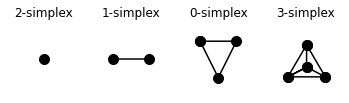
\includegraphics{figures/sections/math/simplex.png}
    \caption{Simplices encode the connectivity of the data, from fully disconnected (0 simplex) observations to all observations are connected to at least 3 other observations. Higher order simplicies are outside the scope of this paper.}
\end{figure}

One way to represent the topological space K is as a set composed of simplices, such as those shown in figure~\ref{fig:simplex}. Simplices are a way of encoding the connectivity of each observation ($\sigma(k)$) to another:

\begin{description}
    \item[0-simplex] discrete observations (inventory records)
    \item[1-simplex] 1D continuos data (timeseries)
    \item[2-simplex] 2D continuos data (map)
    \item[3-simplex] 3D continuos data (video)
\end{description}

In a locally trivial fiber bundle $E = F \times K$, it can be assumed that all $F_{k}$ for $k \in K$ are equal. A fiber bundle can be made locally trivial by approximating the total space E as a simplacial complex.



\subsubsection{Subset \& Streaming}
i for inclusion 
%% insert diagram of U, E, etc

%%% sheaves & presheaves 


\subsection{Visual Space}
%%render image
\begin{tikzcd}
    \mathbb{R}^{7} \arrow[r, hook] & H \arrow[d, "\zeta" description, bend right] \\
                                   & S \arrow[u, "\rho" description, bend right] 
\end{tikzcd}

%%% R7 in H, S base space, mostly will be trivial case H = S\times R^{7}

%% region on screen that corresponds to selection on H that corresponds to selection on S


\subsection{Artist}

\begin{equation}
    A: \Gamma(E) \rightarrow \Gamma(H)
\end{equation}

%%\psi map from S to topological K...
\subsubsection{Visual Idioms: Equivalance class of artists}
Visual Idioms

\subsubsection{Visual Variable Invariance}
Tau can preserves the measurement type properties (group scales)

Will implement in code such that this happens. 


\end{document}